\chapter{The Naive Credal Classifier}

In the simple credal classifier we estimated the lower and upper bounds for each probability separately using our imprecise prior model.
We then used these separate estimates to make inferences about the true probability of interest: $P(c \mid \mathbf{a})$.

However an alternate method for credal classification was proposed by Zaffalon \cite{Zaffalon01} which we will outline in this section.
This classifier is known as the naive Credal classifier (NCC) and can be more determinate than the simple credal classifier we studied earlier.

\section{Previous Work}

Zaffalon has provided multiple examples of this classifier in action.

In one such study he applies the naive Credal classifier to dementia diagnosis \cite{Zaffalon03}.
He starts with a data set containing test results for 3385 different patients split in to five different categories (four describing types of dementia sufferers, one describing healthy patients).
The data set also contains missing values for some of the patient's test results.
In the first part of the study he simply distinguishes between dementia sufferers and non-dementia sufferers.
In this part the NCC is able to isolate a single class about 90\% of the time and in these cases is accurate 95\% of the time.
When it fails to isolate a single class the NBC is only able to classify the same object correctly 70\% of the time.
In the second part he limits the study to the type of dementia thus reducing the data set to 1103 observations.
Here we see similarly positive results; when the NCC isolates a single class it is accurate 94\% of the time and when it outputs more than one class the set size is about 2 on average and the true class is in the set 98\% of the time.
This study gives an example when a large data set can lead to the NCC being highly determinate and accurate.

In another study he applies the NCC to environmental mining data \cite{Zaffalon02}.
Here the data falls in to one of four categories however the data set only consists of 155 complete instances which is much closer in size to our insurance problem.
In this study the NCC only produced a single class 60\% of the time and of these classes had a single accuracy of 52\%.
When returning more than one class the true class was contained in the output set 82\% of the time.
In comparison the NBC had an accuracy of 48\% on the whole data set and 43\% on the subset of objects the NCC was indeterminate about.
This provides a good example of a situation where the NCC will withhold judgement due to a lack of information.

\section{Theory}

To define the naive Credal classifier we first rewrite our original definition of credal dominance \cref{Credal Dominance} as:
\begin{equation}
	\frac{P_t(c' \mid \mathbf{a})}{P_t(c'' \mid \mathbf{a})} = \frac{P_t(c')\prod_{i=1}^{k}P_t(a_i \mid c')}{P_t(c'')\prod_{i=1}^{k}P_t(a_i \mid c'')} > 1
\end{equation}
Note that the equality holds because the constant $P(\mathbf{a})$ is cancelled.

If we use the posterior expectation for our parametrisation as an estimate for the probabilities then we arrive at:
\begin{equation}
	\frac{n(c')+st(c')}{n(c'')+st(c'')} \prod_{i=1}^k \frac{n(a_i, c') + st(a_i , c')}{n(c'') + st(c'')} \frac{n(c'') + st(c'')}{n(a_i, c') + st(a_i , c')} > 1
\end{equation}

To determine whether this inequality holds we can solve the optimization problem:
\begin{align}
	\min & \left[ \frac{n(c'')+st(c'')}{n(c')+st(c')} \right]^{k-1} \prod_{i=1}^k \frac{n(a_i, c') + st(a_i , c')}{n(a_i, c'') + st(a_i , c'')} \\
	\text{s.t.} & \sum_{c \in \mathcal{C}} t(c) = 1 \\
	& 0 < t(a_i, c) < t(c)
\end{align}
Then compare the answer to 1.
This is the same optimization problem as described by Zaffalon \cite{Zaffalon01}.

It is possible to manipulate this problem into an format that is is easier to solve.
Firstly note that the minimum is achieved when each $t(a_i, c') \rightarrow 0$ and $t(a_i, c'') \rightarrow t(c'')$ so we can use these values in the objective function.
Furthermore, at the minimum, we have $t(c') = 1 - t(c'')$.
To simplify the problem set $st(c'') = x$ then our optimization problem becomes a problem in a single variable:
\begin{align} \label{Credal Dominance Test}
	\min \quad & f(x) = \left[ \frac{n(c'') + x}{n(c') + s - x} \right]^{k-1} \prod_{i=1}^k \frac{n(a_i, c')}{n(a_i, c'') + x} \\
	\text{s.t.} \quad & 0 < x < s
\end{align}

Before we solve this optimization problem we can rule out an edge case.
If $n(a_i, c')=0$ for any $a_i$ then the $c'$ does not dominate $c''$.
If $n(a_i, c'')=0$ for any $a_i$ then we set $f(0)=10$ to indicate domination is achieved at this point.

Next step is to figure out what the objective function looks like.
Note that it is always positive so if we take the log of $f$ and differentiate we get:
\begin{equation}
	\frac{d\ln(f)}{dx} = \frac{k-1}{n(c'')+x} + \frac{k-1}{n(c')+1-x} - \sum_{i-1}^k \frac{1}{n(a_i, c'') + x}
\end{equation}
Differentiating again gives:
\begin{equation}
	\frac{d^2\ln(f)}{dx^2} = -\frac{k-1}{(n(c'') + x)^2} + \frac{k-1}{(n(c')+1-x)^2} + \sum_{i=1}^k \frac{1}{(n(a_i, c'') + x)^2}
\end{equation}
This is always positive so the objective function is log concave.
As the logarithm is monotone it follows that $f(x)$ is also concave and hence has a single minimum.

If we remove the edge cases described above we are left with the simple problem of finding the maximum of a concave function in a given interval.
To do so we use the fminbound function in the SciPy library which in turn uses Brent's method \cite{fminbound}.

\section{Application}

We will measure the same metrics as previously for this new classifier.
The results from 10-fold cross validation with varying $s$ values are as follow:

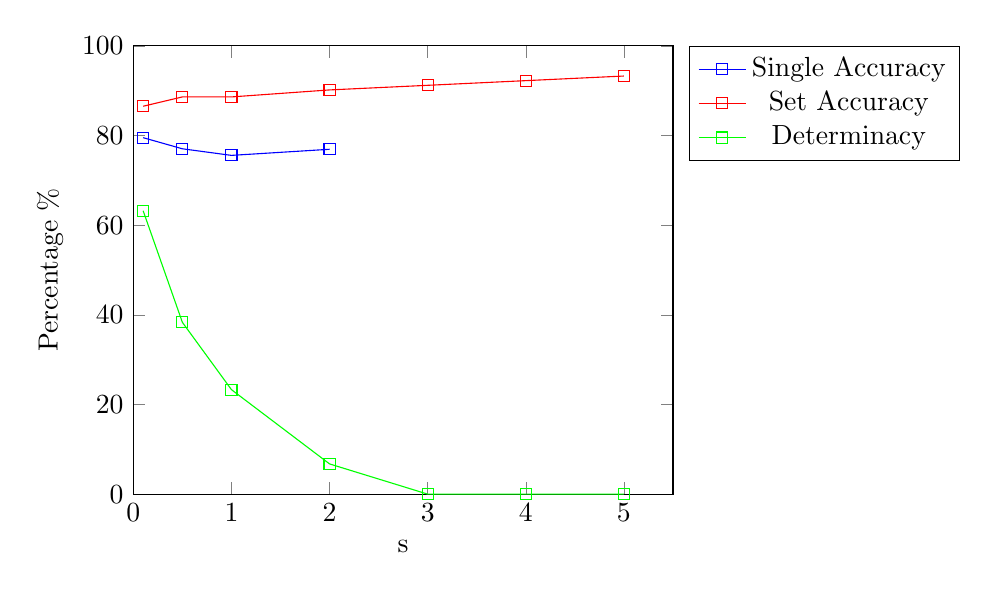
\begin{tikzpicture}
\begin{axis}[
    xlabel={s},
    ylabel={Percentage \%},
    xmin=0, xmax=5.5,
    ymin=0, ymax=100,
	legend pos=outer north east
]

\addplot[
    color=blue,
    mark=square,
    ]
    coordinates {
    (0.1,79.51)(0.5,77.03)(1,75.56)(2,76.92)
    };
    \label{sng_acc}

\addplot[
    color=red,
    mark=square,
    ]
    coordinates {
    (0.1,86.52)(0.5,88.60)(1,88.60)(2,90.16)(3, 91.19)(4, 92.23)(5,93.26)
    };
    \label{set_acc}
 
\addplot[
    color=green,
    mark=square,
    ]
    coordinates {
    (0.1,63.21)(0.5,38.32)(1,23.31)(2,6.74)(3, 0)(4, 0)(5,0)
    };
    \label{det}

\addlegendimage{/pgfplots/refstyle=sng_acc}\addlegendentry{Single Accuracy}
\addlegendimage{/pgfplots/refstyle=set_acc}\addlegendentry{Set Accuracy}
\addlegendimage{/pgfplots/refstyle=det}\addlegendentry{Determinacy}
\end{axis}

\end{tikzpicture}

Additionally we have the following measurements for indeterminate output size:
\begin{center}
\begin{tabular}{c|c c c c}
s & 0.5 & 1 & 2 & 5 \\
\hline
Indeterminate Output Size & 3.65 & 3.66 & 3.74 & 4.25
\end{tabular}
\end{center}

First we note the increase in indeterminate output size and decrease in determinacy.
These are due to the domination criteria becoming harder to satisfy for larger $s$ values.
This leads to less classes being credal dominated and larger output size.

This can also explain the slight trends in single and set accuracy.
Set accuracy increases because the indeterminate output size is always increasing so for each increase in $s$ value we are more likely to see the true class added to the output set if it was not already there.
On the other hand the single accuracy does not change much.
As we increase the $s$ value we decrease the number of single outputs and it would appear the outputs that become indeterminate are equally likely to be correct classifications as incorrect classifications.

We can also directly compare the classifications of the naive Credal classifier to those of our interval based classifier. For $s=1$ we have:
\begin{center}
\begin{tabular}{l|c c c c}
         & A\%     & B\%     & C    & D\%     \\
\hline
Interval & 75.61\% & 89.12\% & 3.71 & 21.32\% \\
NCC      & 75.56\% & 88.60\% & 3.66 & 23.31\% \\
\end{tabular}
\end{center}
Here we see similar set and single accuracies.
However we see that the naive Credal classifier is more determinate than the interval based classifier and, when indeterminate, has a smaller average output size.

Our data set only contains observations of three vehicles with risk rating -2.
This means that our credal classifiers struggle to eliminate this classification as an option.
When we consider situations where the NCC is indeterminate and returns two possible classes -2 is always one of these classes.
Additionally the other class is the correct classification 88.60\% of the time.
These situations demonstrate how the NCC will be indeterminate when there are a small number of observations of a particular class.

\section{Comparison to NBC}

In addition to our interval based credal classifier we can also compare the NCC to the NBC.
We will do this using the same statistics as Zaffalon \cite{Zaffalon01}.
Zaffalon compared the single accuracy of the NCC to the accuracy of the NBC.
He also considered the accuracy of the NBC limited to objects the NCC was indeterminate about.
We will set $s=1$ and consider the same three metrics: NCC single accuracy (A\textsubscript{NCC}\%), NBC accuracy A\textsubscript{NBC} and NBC accuracy on  the NCC's indeterminate objects (A\textsubscript{S}\%).
\begin{center}
\begin{tabular}{c c c}
\hline
A\textsubscript{NCC}\% & A\textsubscript{NBC} & A\textsubscript{s}\% \\
\hline
81.40\%                & 69.43\%              & 66.00\% \\
\hline
\end{tabular}
\end{center}

This demonstrates how the indecisive nature of the naive Credal classifier can hold it back.
We see that when it returns a single class it is far more accurate than the naive Bayes classifier.
However we also see that for objects the NCC is indeterminate about the NBC is only slightly less accurate.
These measurements are in contrast to those achieved by Zaffalon.
When he carried out his analysis he saw that the NBC drop off significantly when only considering the classes the NCC was indeterminate about.

The reason for this difference again comes back to the lack of observations of vehicles with a -2 risk rating.
A lot of the time when the NCC is indeterminate it is only with regards to the true class and the -2 risk rating.
The NBC is more decisive and will opt for the correct class in many of these occasions.

\section{Conclusions}

We have seen that Zaffalon's naive Credal classifier is slightly more determinate than our simple interval based classifier.
We have also seen how our choice of the $s$ hyper parameter affects how cautious our classifier is.

However we have also seen that the naive Credal classifier can be very cautious when there are a small number of observations of a particular class.
We saw that when this is the case it would often return sets of size two containing the true class and the class with a low number of observations.
We saw that this meant the NBC still had a good accuracy when applied to the sets the NCC was indeterminate about because it is a less cautious classifier.